\documentclass[tikz,border=8pt]{standalone}
% Shared look for every TikZ diagram. Load with \input{../../tools/tikz-style.tex}
\usepackage[T1]{fontenc}
\usepackage{lmodern}
\renewcommand{\sfdefault}{lmr}  % diagrams use the same serif as the text
\usetikzlibrary{arrows.meta, positioning, shapes.geometric, calc, fit, backgrounds}
\definecolor{cblue}{HTML}{4C78A8}
\definecolor{corange}{HTML}{F58518}
\definecolor{cgreen}{HTML}{54A24B}
\definecolor{cred}{HTML}{E45756}
\definecolor{cpurple}{HTML}{B279A2}
\definecolor{cgrey}{HTML}{6B6B6B}
\tikzset{
  every picture/.style={font=\sffamily, line width=1.2pt},
  box/.style={draw=#1, fill=#1!12, rounded corners=4pt, align=center, inner sep=7pt, minimum height=1.1cm},
  box/.default=cgrey,
  arrow/.style={-{Stealth[length=3mm]}, draw=cgrey, line width=1.4pt},
  title/.style={font=\sffamily\bfseries\Large},
  note/.style={font=\sffamily\small, text=cgrey, align=center},
}
\AtBeginDocument{\hyphenpenalty=10000 \exhyphenpenalty=10000}

\begin{document}
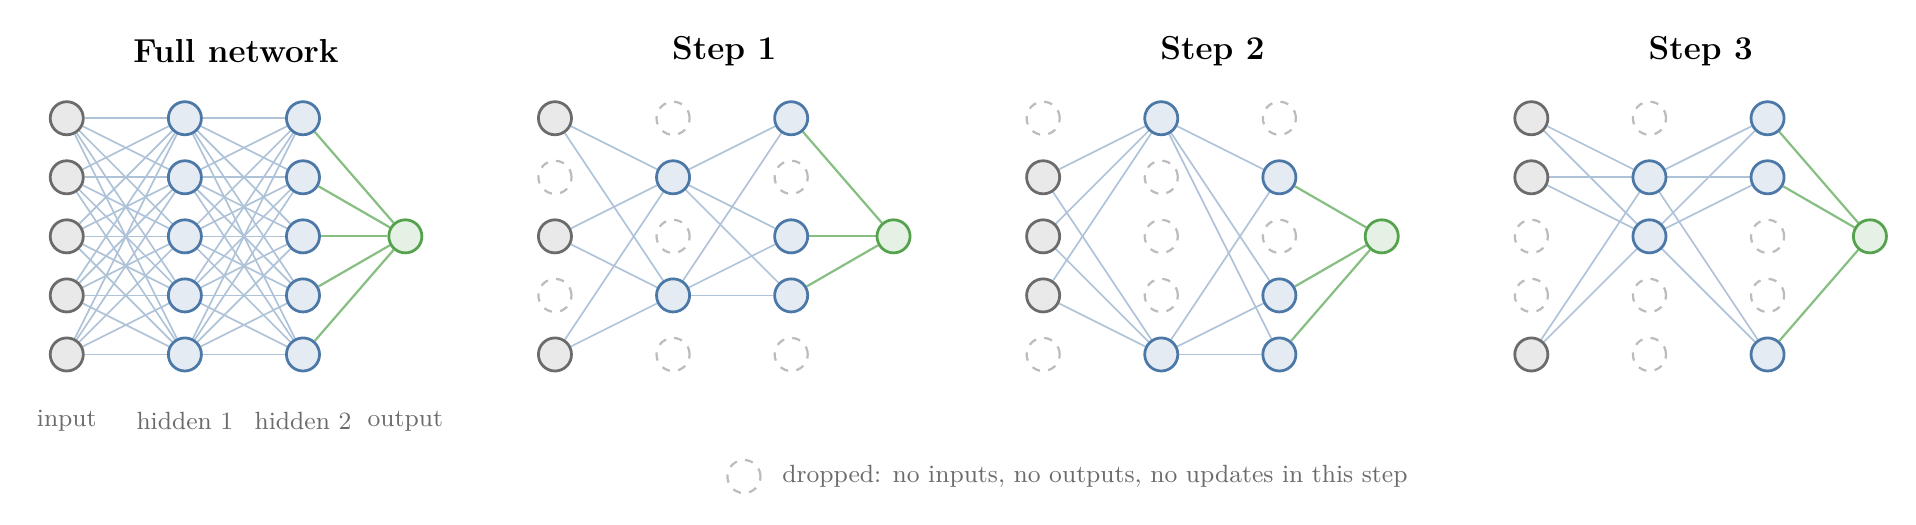
\begin{tikzpicture}[
  on/.style={circle, draw=#1, fill=#1!15, minimum size=0.42cm, inner sep=0pt, line width=1pt},
  off/.style={circle, draw=cgrey!45, fill=white, minimum size=0.42cm, inner sep=0pt, line width=0.8pt, dashed}]
  % one panel: \panel{xshift}{title}{dropped input nodes}{dropped h1 nodes}{dropped h2 nodes}
  \newcommand{\panel}[5]{%
    \begin{scope}[xshift=#1cm]
      \foreach \k in {1,...,5} {
        \def\st{on=cgrey}  \foreach \d in {#3} {\ifnum\d=\k \gdef\st{off}\fi}
        \expandafter\node\expandafter[\st] (i\k) at (0, -0.75*\k) {};
        \gdef\st{on=cblue} \foreach \d in {#4} {\ifnum\d=\k \gdef\st{off}\fi}
        \expandafter\node\expandafter[\st] (h\k) at (1.5, -0.75*\k) {};
        \gdef\st{on=cblue} \foreach \d in {#5} {\ifnum\d=\k \gdef\st{off}\fi}
        \expandafter\node\expandafter[\st] (g\k) at (3.0, -0.75*\k) {};
      }
      \node[on=cgreen] (o) at (4.3, -2.25) {};
      \begin{scope}[on background layer]
        \foreach \i in {1,...,5} \foreach \j in {1,...,5} {
          \def\keep{1}
          \foreach \d in {#3} {\ifnum\d=\i \gdef\keep{0}\fi}
          \foreach \d in {#4} {\ifnum\d=\j \gdef\keep{0}\fi}
          \ifnum\keep=1 \draw[cblue!45, line width=0.6pt] (i\i) -- (h\j); \fi
          \gdef\keep{1}
          \foreach \d in {#4} {\ifnum\d=\i \gdef\keep{0}\fi}
          \foreach \d in {#5} {\ifnum\d=\j \gdef\keep{0}\fi}
          \ifnum\keep=1 \draw[cblue!45, line width=0.6pt] (h\i) -- (g\j); \fi
        }
        \foreach \j in {1,...,5} {
          \gdef\keep{1}
          \foreach \d in {#5} {\ifnum\d=\j \gdef\keep{0}\fi}
          \ifnum\keep=1 \draw[cgreen!70, line width=0.8pt] (g\j) -- (o); \fi
        }
      \end{scope}
      \node[font=\sffamily\bfseries\large] at (2.15, 0.1) {#2};
    \end{scope}}
  \panel{0}{Full network}{0}{0}{0}
  \panel{6.2}{Step 1}{2,4}{1,3,5}{2,5}
  \panel{12.4}{Step 2}{1,5}{2,3,4}{1,3}
  \panel{18.6}{Step 3}{3,4}{1,4,5}{3,4}
  \node[note] at (0, -4.6) {input}; \node[note] at (1.5, -4.6) {hidden 1};
  \node[note] at (3.0, -4.6) {hidden 2}; \node[note] at (4.3, -4.6) {output};
  \node[circle, draw=cgrey!45, dashed, line width=0.8pt, minimum size=0.42cm] at (8.6, -5.3) {};
  \node[note, anchor=west] at (8.95, -5.3) {dropped: no inputs, no outputs, no updates in this step};
\end{tikzpicture}
\end{document}
